\section{CNNDroid}
CNNDroid is an open source deep learning library for Android. It is able to execute convolutional neural networks, supporting most CNN layers used by existing desktop/server deep learning frameworks, namely Caffe, Theano and Torch. Supported layers, as of March 2017 are:
\begin{itemize}
    \item{Convolutional Layer}
    \item{Pooling Layer}
    \item{Local Response Normalization Layer}
    \item{Fully-Connected Layer}
    \item{Rectified Linear Unit Layer (ReLU)}
    \item{Softmax Layer}
    \item{Accuracy and Top-K Layer}
\end{itemize}
Due to the library being open source, it is possible to add additional layers, such as batch normalization or sigmoid.\\
The library also supports a variety of customizations, like maximum memory usage, GPU or CPU acceleration and automatic performance tuning.

\subsection{Setup and Integration into Android Project}
CNNDroid is a source code library. That means that integration into an existing Android Project is fairly straight forward and doesn't require any third-party dependencies.\\
The only prerequisites are:
\begin{itemize}
    \item{A functional Android development environment (e.g. Android Studio\footnote{\url{https://developer.android.com/studio/index.html}})}
    \item{Android phone or emulator running at least Android SDK version 21.0 (Lollipop)}
\end{itemize}

To integrate CNNDroid into the project, the project has to be cloned from its GitHub\footnote{https://github.com/ENCP/CNNdroid} page. Inside the `\texttt{CNNdroid Source Package}' folder, there are three folders. `\texttt{java}', `\texttt{rs}' and `\texttt{libs}'.\\
The `\texttt{java}' and `\texttt{rs}' folders need to be copied into the your `\texttt{app/src/main/}' directory, merging the `\texttt{java}' folders.\\
The `\texttt{libs}' folder has to be copied and merged into your `\texttt{app/}' directory.\\
For effective usage of CNNDroid, it needs read and write access to storage on the smartphone. Android policies require an application to request these permissions before the app starts. These permission requests are specified inside the `\texttt{AndroidManifest.xml}' file. Inside this file, the following lines have to be added before the `\lstinline[language=XML]{<application}' section:

\begin{lstlisting}[language=XML, basicstyle=\scriptsize]
    <uses-permission android:name="android.permission.READ_EXTERNAL_STORAGE"/>
    <uses-permission android:name="android.permission.WRITE_EXTERNAL_STORAGE"/>
\end{lstlisting}

To cope with the high computational requirements, CNNDroid potentially needs a large amount of memory. Therefore, the heap has to be increased, which is done by adding

\begin{lstlisting}[language=XML, basicstyle=\scriptsize]
    android::largeHeap="true"
\end{lstlisting}
\noindent
inside the `\lstinline[language=XML]{<application}' section.\\
Now, everything should be set up correctly and programming can commence.\\
After importing the package \lstinline[language=Java]{network.CNNdroid}, the \lstinline[language=Java]{CNNdroid} object is accesible, which can call the function \lstinline[language=Java]{CNNDroid::classify}. This is the keyword to start execution of the trained model. The specification of the model is explained in the following section.

\subsection{Structure Overview of necessary CNNDroid Files}
Of course, CNNDroid needs to know how to classify an input. For that it either uses converted binary layer files, created by a desktop deep learning framework or internal conversion functions (e.g. for pooling or ReLU).\\
The layer blobs are generally used for more complicated layers, such as convolutional or fully connected layers, which have a high dimensional and variable amount of variables. These files have to be converted into the MessagePack\footnote{http://msgpack.org/} format and put onto the smartphones storage.\\
The order in which the layers are executed, additional configurations and layers which don't need a blob file are defined inside the definition file. This file is used as a settings file for the \lstinline[language=Java]{CNNdroid} classifier.\\
On creation of the \lstinline[language=Java]{CNNdroid} object, the absolute path to this file has to be specified.\\
Configurations, other than the layer definitions are:
\begin{itemize}
    \item{the absolute path to the layer blob files\\(\lstinline[language=Java]{root_directory: "/absolute/path/to/layer/files"})}
    \item{the maximum amount of RAM the classifier should use on the smartphone\\(\lstinline[language=Java]{allocated_ram: Amount_in_MB})}
    \item{whether or not automatic performance tuning should be used\\(\lstinline[language=Java]{auto_tuning: "on|off"})}
    \item{whether or not classification should be GPU accelerated (if possible)\\(\lstinline[language=Java]{execution_mode: "sequential|parallel"})}
\end{itemize}
Layers are defined as shown in figure \ref{fig:def_file}.

\begin{figure}
  \centering
    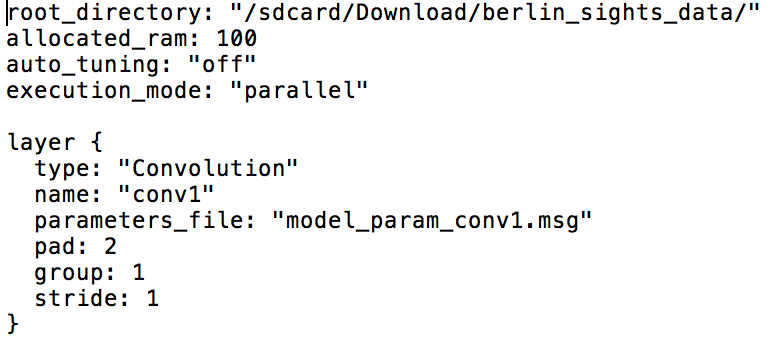
\includegraphics[width=0.5\textwidth]{def_file.png}
  \caption{Excerpt of a CNNDroid definition file}
  \label{fig:def_file}
\end{figure}

Not essential for the execution of CNNDroid, but very helpful for processing the final results, is a labels file. This file should specify human-readable names for the extractable classes. The order inside this file should be mapped to the output order of the last layer (probably a fully-connected layer), i.e. the first value of the output array should correspond to the first class name inside the labels file.

\subsection{Convert Trained Models into CNNDroid-compatible Format}
Short Introduction to MessagePack
\begin{itemize}
    \item{how to use convertion script}
    \item{compatible frameworks}
    \item{compatible layers}
\end{itemize}

\subsection{CPU vs GPU performance}
Comparison of computation time of CPU (sequential) and GPU (parallel) mode on in-memory images using CIFAR10 (in-memory to minimize error using camera, CIFAR10 could be exchanged with CaffeNet if too fast)